\section{Tablas de verdad}
\subsection{Escribir las tablas de verdad de las funciones lógicas siguientes:} 
and, xor, or, xnor, nand, not y nor.

\begin{multicols}{4}

% --- AND ---
\subsection*{AND}
\begin{tabular}{c c | c}
\toprule
A & B & X \\
\midrule
0 & 0 & 0 \\
0 & 1 & 0 \\
1 & 0 & 0 \\
1 & 1 & 1 \\
\bottomrule
\end{tabular}

% --- XOR ---
\subsection*{XOR}
\begin{tabular}{c c | c}
\toprule
A & B & X \\
\midrule
0 & 0 & 0 \\
0 & 1 & 1 \\
1 & 0 & 1 \\
1 & 1 & 0 \\
\bottomrule
\end{tabular}

% --- OR ---
\subsection*{OR}
\begin{tabular}{c c | c}
\toprule
A & B & X \\
\midrule
0 & 0 & 0 \\
0 & 1 & 1 \\
1 & 0 & 1 \\
1 & 1 & 1 \\
\bottomrule
\end{tabular}

% --- XNOR ---
\subsection*{XNOR}
\begin{tabular}{c c | c}
\toprule
A & B & X \\
\midrule
0 & 0 & 1 \\
0 & 1 & 0 \\
1 & 0 & 0 \\
1 & 1 & 1 \\
\bottomrule
\end{tabular}

% --- NAND ---
\subsection*{NAND}
\begin{tabular}{c c | c}
\toprule
A & B & X \\
\midrule
0 & 0 & 1 \\
0 & 1 & 1 \\
1 & 0 & 1 \\
1 & 1 & 0 \\
\bottomrule
\end{tabular}

% --- NOT ---
\subsection*{NOT}
\begin{tabular}{c | c}
\toprule
A & X \\
\midrule
0 & 1 \\
1 & 0 \\
\bottomrule
\end{tabular}

% --- NOR ---
\subsection*{NOR}
\begin{tabular}{c c | c}
\toprule
A & B & X \\
\midrule
0 & 0 & 1 \\
0 & 1 & 0 \\
1 & 0 & 0 \\
1 & 1 & 0 \\
\bottomrule
\end{tabular}

\end{multicols} 

\begin{verbatim}
       |\      _,,,---,,_
ZZZzz /,`.-'`'    -.  ;-;;,_
     |,4-  ) )-,_. ,\ (  `'-'
    '---''(_/--'  `-'\_)
\end{verbatim}

\subsection{Escribir la tabla de verdad del siguiente diagrama de compuertas lógicas:}

\begin{figure}[H]
    \centering
    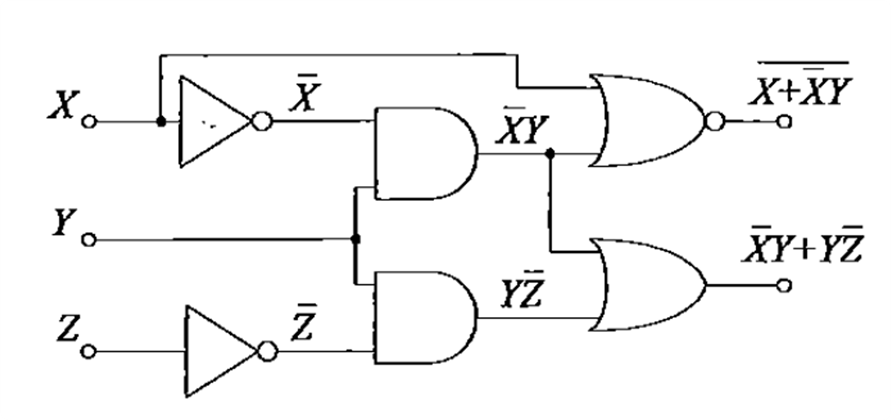
\includegraphics[width=0.5\linewidth]{Puertas lógicas.png}
    \caption{Diagrama de compuertas lógicas}
    \label{fig:puertas}
\end{figure}

\begin{table}[h]
\centering
\begin{tabular}{c c c | c | c }
\toprule
X & Y & Z & $\overline{ X + \overline{X}Y}$ & $\overline{X}Y + Y \overline{Z} $ \\
\midrule
0 & 0 & 0 & 1 & 0 \\
0 & 0 & 1 & 1 & 0 \\
0 & 1 & 0 & 0 & 1 \\
0 & 1 & 1 & 0 & 1 \\
1 & 0 & 0 & 0 & 0 \\
1 & 0 & 1 & 0 & 0 \\
1 & 1 & 0 & 0 & 1 \\
1 & 1 & 1 & 0 & 0 \\
\bottomrule
\end{tabular}
\end{table}

\subsection{Llenar la siguiente tabla según corresponda.}

\begin{table}[h]
\centering
\begin{tabular}{| c | c | c |}
\toprule
Decimal & Binario & Hexadecimal \\
\midrule
\textbf{1230} & \textbf{0100 1100 1110} & \textbf{4CE} \\
1433 & \textbf{0101 1001 1001} & 599 \\
1532 & 0101 1111 1100 & \textbf{5FC} \\
\textbf{1141} & 0100 0111 0101 & 475 \\
3864 & \textbf{1111 0001 1000} & F18 \\
3770 & 1110 1011 1010 & \textbf{EBA} \\
\textbf{1023} & 0011 1111 1111 & 3FF \\
352 & \textbf{0001 0110 0000} & 160 \\
2582 & 1010 0001 0110 & \textbf{A16} \\

\bottomrule
\end{tabular}
\end{table}

\newpage

\subsection*{Conversiones de Decimal a Binario y Hexadecimal}

\subsubsection*{1. Decimal: 1230}

\textbf{Decimal $\to$ Binario:}

\[
\begin{array}{c|c|c}
\text{División} & \text{Cociente} & \text{Resto} \\
\hline
1230 \div 2 & 615 & 0 \\
615 \div 2 & 307 & 1 \\
307 \div 2 & 153 & 1 \\
153 \div 2 & 76 & 1 \\
76 \div 2 & 38 & 0 \\
38 \div 2 & 19 & 0 \\
19 \div 2 & 9 & 1 \\
9 \div 2 & 4 & 1 \\
4 \div 2 & 2 & 0 \\
2 \div 2 & 1 & 0 \\
1 \div 2 & 0 & 1 \\
\end{array}
\]

\[
\text{Binario: } 0100\,1100\,1110
\]

\textbf{Binario $\to$ Hexadecimal:}

0100 = 4

1100 = C

1110 = E

\[
\text{Hexadecimal: } 4CE
\]

\subsubsection*{2. Binario: 0101 1001 1001}

\textbf{Binario $\to$ Decimal:}

\[
1\cdot2^0+0\cdot2^1+0\cdot2^2+1\cdot2^3+ 1\cdot2^4+0\cdot2^5+0\cdot2^6+1\cdot2^7 +1\cdot2^8+0\cdot2^9+1\cdot2^{10}+0\cdot2^{11} 
\]

\[
 = 2^0 + 2^3 + 2^4 + 2^7 + 2^8+2^{10}
\]

\[
 = 1 + 8 + 16 + 128 + 256 + 1024 
\]

\[
 = 153 + 1280  
\]

\[
 = 1433  
\]

\[
\text{Decimal: } 1433
\]

\textbf{Binario $\to$ Hexadecimal:}

0101 = 5

1001 = 9

1001 = 9

\[
\text{Hexadecimal: } 599
\]

\subsubsection*{3. Hexadecimal: 5FC}

\textbf{Hexadecimal $\to$ Binario:}

5 = 0101

F = 1111

C = 1100

\[
\text{Binario: } 0101\,1111\,1100
\]

\textbf{Binario $\to$ Decimal:}

\[
 = 0\cdot 2^0 + 0\cdot 2^1 + 1\cdot 2^2 + 1\cdot 2^3
 + 1\cdot 2^4 + 1\cdot 2^5 + 1\cdot 2^6 + 1\cdot 2^7
 + 1\cdot 2^8 + 0\cdot 2^9 + 1\cdot 2^{10} + 0\cdot 2^{11}
\]

\[
 = 2^2 + 2^3 + 2^4 + 2^5 + 2^6 + 2^7 + 2^8 + 2^{10}
\]

\[
 = 4 + 8 + 16 + 32 + 64 + 128 + 256 + 1024 
\]

\[
\text{Decimal: }  1532
\]